\documentclass[a4paper,11pt]{custom}
\usepackage[utf8]{inputenc}
\usepackage[T1]{fontenc}
\usepackage[left=2.5cm,right=2.5cm]{geometry}
\usepackage{indentfirst}
\usepackage[official]{eurosym}
\usepackage{relsize}

%
%--------------------   start of the 'preamble'
%
\usepackage{graphicx,amssymb,amstext,amsmath,multicol,wrapfig}
%
%%    homebrew commands -- to save typing
\newcommand\etc{\textsl{etc}}
\newcommand\eg{\textsl{eg.}\ }
\newcommand\etal{\textsl{et al.}}
\newcommand\Quote[1]{\lq\textsl{#1}\rq}
\newcommand\fr[2]{{\textstyle\frac{#1}{#2}}}
\newcommand\miktex{\textsl{MikTeX}}
\newcommand\comp{\textsl{The Companion}}
\newcommand\nss{\textsl{Not so Short}}
%
%---------------------   end of the 'preamble'
%
\newcommand{\smu}{\textsc{Smart Me Up}}

\newcommand{\rtp}{\textbf{rtp}}
\newcommand{\rtcp}{\textbf{rtcp}}
\newcommand{\rtsp}{\textbf{rtsp}}

\newcommand{\vlc}{\textbf{vlc}}
\newcommand{\avconv}{\textbf{avconv}}
\newcommand{\ffmpeg}{\textbf{ffmpeg}}
\newcommand{\gstreamer}{\textbf{gstreamer}}
\newcommand{\curl}{\textbf{curl}}
\newcommand{\boost}{\textbf{boost}}
\newcommand{\happyhttp}{\textbf{HappyHTTP}}
\newcommand{\libcurl}{\textbf{libcurl}}

\newcommand{\mjpeg}{\textbf{mjpeg}}
\newcommand{\jpeg}{\textbf{jpeg}}
\newcommand{\vpx}{\textbf{vp8}}
\newcommand{\mpeg}{\textbf{h264}}

\newcommand{\cmake}{\textbf{cmake}}
\newcommand{\jni}{\textbf{jni}}
\newcommand{\fpm}{\textbf{fpm}}

\newcommand{\rpi}{\textbf{raspberry pi}}
\newcommand{\bbb}{\textbf{beaglebone black}}

\newcommand{\linux}{\textbf{Linux}}
\newcommand{\win}{\textbf{Windows}}
\newcommand{\mac}{\textbf{Mac}}
\newcommand{\android}{\textbf{Android}}
\newcommand{\ios}{\textbf{iOS}}

\newcommand{\claude}{\textit{Claude}}

\newcommand{\nth}[1]{#1$^{\text{\tiny th}}$}
\newcommand{\second}{2$^{\text{\tiny nd}}$}

%C plus plus
\newcommand{\cpp}{%
  C\kern-.1667em\raise.30ex\hbox{\smaller{++}}%
  \spacefactor1000%
}
\newcommand{\json}{\textbf{json}}

\setlength{\parskip}{1em}

\begin{document}
%-----------------------------------------------------------

% \section La page de couverture du rapport (dont vous trouverez un modèle sur 
% l¿intranet) doit comporter obligatoirement les informations suivantes:

% \item le nom et prénom du stagiaire
% \item l'indication "stage de deuxième année"
% \item le nom de l¿enseignant scientif i que membre du jury
% \item le nom et l'adresse de la structure d¿accueil
% \item les dates de début et de fi n du stage, et sa durée
% \item le sujet du stage

\title{
  Live video streaming
}
\author{
  Robin Moussu 2A SLE
  \thanks{
  \begin{tabular}{c}
    \textit{Intership of 2$^{nd}$ year as}\\
    \textit{engineer assistant}\\
    \vspace{2em}\\
    \begin{tabular}{rcl}
      15 june &--& 15 september\\
      \multicolumn{3}{c}{3 months}\\
      \\
      tutor &--& Olivier Kilh \\
      supervised by &--& Steven Durand \\
      ensimag tutor &--& Roland Groz\\
      \\
    \end{tabular}
    \vspace{2em}\\
    \smu\\
    4 chemin des prés\\
    Meylan\\
  \end{tabular}
  }
}
\date{
  September, 2015
}
\maketitle

%-----------------------------------------------------------

~
\thispagestyle{empty}

\headerdecoration[-.5cm]{PaleTurquoise}%
\headerleftcontent{\headerlefttext}%
\headerrightcontent{\headerrighttext}%
\myfootrulebegin[-.5cm]
\myfootruleend

~

\clearpage

\pagenumbering{arabic}

~

\vspace{\fill}
\begin{flushright}
\begin{minipage}[b]{7cm}
I want to thanks warmly M. Steven Durand (CTO) and M. Loïc Lecerf (CEO) for
guiding me during my intership, together with M. Olivier Kilh my tutor.

\vspace{0.5em}

My thanks also goes to all the employes and interns of \smu, especialy Maude
Premillieu and Gabriel Mattos Langeloh. It was realy a pleasant experience to
work with them.
\end{minipage}
\end{flushright}
\vspace{\fill}
\vspace{\fill}


\newpage
~
\newpage

%-----------------------------------------------------------
%\chapterimage{nature-clouds-hdr-phenomenon.jpg}
%\tableofcontents
%-----------------------------------------------------------
%\chapterimage{binary.jpg}
%\chapter{Introduction}
The first chapter of a well-structured report is always an
introduction, setting the scene with motivation and context (as in
Sec.~\ref{intro}) and then looking ahead to summarise what's in the
rest of the report (as in Sec.~\ref{intro:contents}). It's the
bit that readers look at first --- {\em so make sure it hooks them!}
%
\section{Context and motivation}\label{intro}
This is a template for \LaTeX\ project reports in the Department of
Mathematical Sciences. It shows a good overall structure for the
printed document, and shows how to construct it with a master file
(\texttt{report.tex}) plus subsidiary files (\texttt{chap1.tex},
\dots, \texttt{app1.tex}, \dots, \texttt{biblio.tex}).
\par
At the same time, features of the current version of \LaTeX\ (\LaTeXe)
are illustrated --- such as mathematical expressions, numbering and
cross-referencing, bibliography and citations, graphics and tables.
Comparison of the source files with the printer-ready document will
answer a few FAQs: \Quote{How can I do \dots\ in \LaTeX?}.
\par
However, this is {\em not} a textbook on \LaTeX\ --- for that, use the
\lq\nss\rq\ notes by Oetiker \etal\ \cite{NSS}. They are written for
novices, and are a pleasure to read. They are available free on-line,
and are kept up-to-date. The \LaTeX\ book at \textsl{Wikipedia}
\cite{WL} includes the \nss\ material and is good for reference too.
Access these via the \LaTeX\ resources page \cite{LAT}.
\par
For more advanced features see \eg\lq\comp\rq\ \cite{MG}.
\par
Well-meant advice on \LaTeX\ for report-writing and poster-making is
available\footnote{From  \texttt{bob.johnson@dur.ac.uk}} in room CM315,
where there are reference copies of both \comp\ \cite{MG} and
\textsl{The Graphics Companion} \cite{GRM}.
\par
Even if you are misguided enough \cite{AC} to prepare your report in
\textsl{Word}, this template at least exemplifies a good structure ---
and gives advice about references and help with typography.
%
\section{Contents}\label{intro:contents}
The main body of this report is divided as follows.
\par
Chap.~\ref{sec:formulas} has some examples of mathematics, then
Chap.~\ref{sec:graphics} deals with graphics and includes
Sec.~\ref{sec:tables} about tables. The Conclusion, in
Chap.~\ref{andfinally}, summarises what's been achieved, the open
questions and what could be done next.
\par
Then comes the Bibliography, listing all sources of material, data and
computer programs used, \etc. Its construction is explained in
\cite[Sec.~4.2]{NSS} and there's more about it in App.~\ref{app:refs}.
\par
Otherwise appendices typically hold basic background theory, or
additional or similar examples, or longer proofs (App.~\ref{app:proofs})
 --- anything you need but which would hold up the main flow of the
story. You could also use an appendix for listings of any computer
programs that you've written (App.~\ref{app:programs}).
\par
Here there's information about using a PC (App.~\ref{app:pc}) plus
brief advice on grammar and typography (App.~\ref{app:typo}).
%

%\chapterimage{Raspberry_Pi_2.jpg}
%\chapter{Formulas and theorems}\label{sec:formulas}
Each main chapter or section should start with a short description of
what it holds, and why. Top tip --- begin the whole writing enterprise
with a first draft of this little bit for each chapter. It will force
you to think about overall structure.
\par
Here we get going with mathematics and show firstly some simple
equations and then some that are slightly less simple. Then there's a
theorem whose proof is relegated to an appendix, followed by some
numbered results.
%
\section{Plain}
Here's an inline formula: \(E=mc^2\), and here's the same
thing displayed:\[E=mc^2.\]A matrix needs to be displayed:
\[  \det\left(\begin{array}{cc}
        a & b \\  c & d \\
      \end{array}\right) = ad-bc,   \]
and here's a result that's displayed and labelled:
\begin{equation}\label{eq:display}
\lim_{a\to\infty}\int_0^a\exp(-x^2)\,dx=\fr12\sqrt\pi.
\end{equation}Note the punctuation in eq.~(\ref{eq:display}) \etc,
which recognises that displayed equations are parts of sentences.
\par
Note also that a smaller (\verb+\textstyle+) size of numerical fraction
is often useful in a displayed equation. The appropriate
\verb+\newcommand+ called \verb+\fr+ is defined in the
\Quote{preamble}, in file \texttt{report.tex}.
\par
More complicated limits on \verb+\int+ (and \verb+\sum+) need to
be enclosed in braces $\{\cdots\}$.
\par
In an inline formula, avoid ugly fractions such as \(v=\frac st\) and
\(\frac{dy}{dx}=x+y\). It looks much better to write \(v=s/t\) and
\(dy/dx=x+y\). That is, keep \verb+\frac+ for
display:\[\frac{dy}{dx}=x+y\]where it belongs.
\par
Beware of inadvertent blank lines in your \texttt{.tex} file; they often
creep in immediately after a displayed equation. A blank line gives a
new paragraph, usually indented, which may not be what you want. You can 
avoid blank lines altogether by breaking paragraphs with \verb+\par+
instead, as done here.
%
\section{Fancy}
Now an equation on several lines using \verb+align+:
\begin{align*}
  |\vec A|^2 &= a_1^2+a_2^2  \\
             &= \sin^2\theta+\cos^2\theta \\
             &= 1
\end{align*}--- where the star on \verb+align*+ suppresses
all line-numbering\footnote{And re-phrase material where any displayed
equation splits between pages.}.
\par
Again, with just one line numbered for reference:
\begin{equation}
\begin{aligned}
  |\vec A|^2 &= a_1^2+a_2^2  \label{line-one}\\
             &= \sin^2\theta+\cos^2\theta \\
             &= 1 
\end{aligned}
\end{equation}
Now you can refer to equation~(\ref{line-one}).
\par
If you want to number the equations in Chapter 2 as (2.1), (2.2), etc,
then\footnote{Top tip: easily find out about any \LaTeX\ command by
putting it \textit{with} its backslash (and perhaps the word \lq latex')
into your favourite search engine.} put \lq\verb+\numberwithin+' into
\textsl{Google} or see \cite[Sec 8.2.14]{MG}.
\par
Notice that in equations you use \verb+\lim+, \verb+\exp+, \verb+\sin+
and \verb+\cos+ and not plain $lim$, $exp$, $sin$ and $cos$. See
\cite[Sec.~3.3]{NSS} for a list.
\par
For a lot of complicated multi-line formulas it's better to use the more
sophisticated display environments provided by the package
\texttt{amsmath} --- see Sec.~8.2 of \comp\ \cite{MG}.
For instance the \texttt{cases} environment is used to get
\[\theta(x)=\begin{cases}0&\text{if $x<0$,}\\
		1&\text{if $x>0$.}\end{cases}\]
And if you need continued fractions, instead of 
\[x=\frac{1}{a_2+\frac{1}{a_3+\frac{1}{a_4+\cdots}}},\]a better-looking
result
is\[x=\frac{\strut1}{\displaystyle a_2+\frac{\strut1}{\displaystyle
a_3+\frac{\strut1}{\displaystyle a_4+\cdots}}},\]for which
\texttt{amsmath}
provides the command \verb+\cfrac+ \cite[Sec.~8.4.2]{MG}.
\par
The package \texttt{amssymb} \cite[Chap.~8]{MG} extends the range of
mathematical symbols (\eg\(\mathbb{R}\), \(\mathbb{Z}\) and
\(\mathbb{N}\) are available).
\par
And its sister \texttt{amstext} provides the command \verb+\text+ to
put words into a displayed equation \[ \text{like this: }E=mc^2. \]Note
that you need to put in by hand the spacing between the text and the
mathematical symbols.
%
\section{Theorems}\label{angels}
This is theorem~\ref{angels}.
\begin{description}
\item[Theorem]: The whole is greater than the sum of its parts.
\item[Proof:] See App.~\ref{app:proofs}, Sec.~\ref{pf:angels}.
\end{description}
For numbered theorems, use \verb+\newtheorem+ \cite[Sec.~3.8]{NSS}.
\par
Here's the main sequence of theorems.
\newtheorem{Main}{Theorem} % this could go into the preamble
\begin{Main}[my first result]
The first theorem, showing
\[ \bar D^n\quad\text{and}\quad\bar{D^n} \]
where the first bar is over just the \lq D\rq\ and the second is over
the whole expression. Also the word \lq and\rq\ is inside displayed
maths, using \verb+\text+ with extra space before and after.
\end{Main}And that's how to do left and right quotation marks, too,
with \verb+\lq+ and \verb+\rq+.
\begin{Main}
The second theorem --- with \verb+\overline+ inline: $\overline{D^n}$.
\end{Main}
\begin{Main} the third theorem\end{Main}
Here's another sequence of results.
\newtheorem{second}{Lemma} % this too could go into the preamble
\begin{second}[my second result]
The next result (a mere lemma) \dots\end{second}
\begin{second}\dots\ and the next\end{second}
\comp\ \cite[Sec.~3.3.3]{MG} describes how to use the
packages \texttt{amsmath} and \texttt{amsthm} to state (and
cross-reference) theorems, lemmas, definitions, proofs, \etc\ in a more 
sophisticated way.
%
\section{Summary}
Each chapter should end with a round-up of its contents and a link
with the contents of the next.
\par
After formulas, equations and theorems, the next important
topics are graphics and tables.

%\chapterimage{webcams.jpg}
%include{chap3}
%\chapterimage{Spider_web_necklace_with_pearls_of_dew.jpg}
%\chapter{Conclusion}\label{andfinally}
The last chapter of a well-structured report reviews what's been done and
mentions the main open questions.  It's the part a typical reader looks
at second, after the Introduction, and it should be just as appealing.
\par
This template is provided only to help you start with \LaTeX\ and to
exemplify good structure. When you've got some practice, you'll want to
alter it to suit your topic and your taste --- and you are free to do
that.
\begin{itemize}
    \item\verb+\documentclass[a4paper,twocolumn,10pt]{article}+
    gives an attractive alternative framework, for example.\par Or you
may prefer \verb+\documentclass{memoir}+ which has an excellent
manual \cite{MEM} that includes a general introduction to typography.
    \item Try to resist the temptation to make margins narrower
    and lines longer --- it may save a sheet or two of paper but it
    can make the text hard to read. Indeed, typesetting professionals 
    quote a maximum of 66 characters per line as an ideal for easy reading
          \cite[Sec.~5.2.2]{NSS}.
    \item proof-read carefully --- not only to get the best from \LaTeX\
but also to polish grammar, spelling and punctuation \cite{ESL}.
App.~\ref{app:typo} alerts you to common pitfalls.
\end{itemize}
Good layout and use of \LaTeX, plus fluent and grammatical writing, will
together give a very good impression.
\par
Top tip --- write what you think is the final version, then put it
away in a drawer and come back to it a week or so later. With fresh
eyes you'll see many potential improvements. This works for anything you
prepare, not just a project report. It needs forward planning of
course!
\section*{Acknowledgements}
\addcontentsline{toc}{chapter}{\numberline{}Acknowledgements}
Here's the place for thanks to anyone who particularly helped you.
Don't go too far OTT --- try to keep some dignity. This isn't the 
Oscars.


%-----------------------------------------------------------
%\chapterimage{Pink_flowers.jpg} % Table of contents heading image
%\addcontentsline{toc}{chapter}{\numberline{}Bibliography}
%\begin{thebibliography}{9999}%\enlargethispage{\baselineskip}
\bibitem[AC]{AC}A~Cottrell, \textsl{Word Processors: Stupid and
Inefficient},
\\ \mbox{}\hfill\texttt{www.ecn.wfu.edu/\~{}cottrell/wp.html}
\bibitem[BR]{BR}Visit \texttt{www.dur.ac.uk/library/using/guides/}
and click on \Quote{Writing your bibliography and citing references}.
\bibitem[ESL]{ESL}L~Truss, \textsl{Eats, Shoots and Leaves}, Profile
  Books 2003\\ \mbox{}\hfill(ISBN~\texttt{1-86197-612-7}).
\bibitem[GRM]{GRM}M~Goossens, S~Rahtz and F~Mittelbach,\\
  \mbox{}\hfill \textsl{The \LaTeX\ Graphics Companion},
  Addison-Wesley, 1997\\  \mbox{}\hfill(ISBN~\texttt{0-201-85469-4}).
\bibitem[IM]{IM} \textsl{ImageMagick}, {\tt%
www.dur.ac.uk/its/software/application/\dots
\\ \mbox{}\hfill\dots?application=ImageMagick}
\bibitem[LAT]{LAT} \textsl{\LaTeX\ stuff},
	\texttt{maths.dur.ac.uk/Ug/projects/resources/latex/}
\bibitem[MEM]{MEM} \textsl{Memoir document class},\\ \mbox{}\hfill
   \texttt{www.ctan.org/tex-archive/macros/latex/contrib/memoir/}
\bibitem[MG]{MG}F~Mittelbach and M~Goossens \etal, \textsl{The
\LaTeX\ Companion},\\  \mbox{}\hfill Addison-Wesley, 2nd ed. 2004
(ISBN~\texttt{0-201-36229-6}).
\bibitem[MKT]{MKT} \textsl{MikTex Project Page}, \texttt{www.miktex.org}
\bibitem[NSS]{NSS}T~Oetiker, H~Partl, I~Hyna and E~Schlegl,\\
\mbox{}\hfill
\textsl{The Not So Short Introduction to \LaTeXe},\\ \mbox{}\hfill{\tt
www.ctan.org/tex-archive/info/short}
\bibitem[PS]{PS} \textsl{Photoshop}, {\tt%
www.dur.ac.uk/its/software/application/\dots
\\ \mbox{}\hfill\dots?application=Adobe+Photoshop}
\bibitem[TXC]{TXC} \textsl{TeXnicCenter}, \texttt{www.toolscenter.org}
\bibitem[WDT]{WDT} \textsl{WinEdt}, \texttt{www.winedt.com}
\bibitem[WL]{WL} \textsl{Wikibook on \LaTeX}, \texttt{%
	en.wikibooks.org/wiki/Latex}
\bibitem[WO]{WO} \textsl{Controlling widows and orphans}, 
\\ \mbox{}\hfill\texttt{www.tex.ac.uk/cgi-bin/texfaq2html?label=widows}
\bibitem[WSH]{WSH} \textsl{WinShell}, \texttt{www.winshell.de}
\end{thebibliography}
\vfill
\begin{flushright}\small Prepared in \LaTeXe\ by RCJ\end{flushright}

%-----------------------------------------------------------
%\appendix
%\chapter{Long proofs}\label{app:proofs} An Appendix is a good place
to put lengthy proofs that must be included but would impede the
flow if placed in the main text.
\section{Proof of theorem \ref{angels}}\label{pf:angels}
By inspection.

%\chapter{Computer programs}\label{app:programs}
An Appendix is the place to list computer programs that you've
written, using the {\tt verbatim} environment \cite[Sec.~2.11.4]{NSS}.
\par
For example ---
\begin{verbatim}
    10 PRINT "HALLO SAILOR!"
    20 GO TO 10
\end{verbatim}

%\chapter{About references}\label{app:refs}
Your report will be put together in your own style, mostly using your
own words. Much of it will be standard material that you've read and
digested, but you may have a fresh example, application or calculation
that you've done yourself.
\par
You must make clear what's not your own work by referring suitably
to your sources --- books or articles or web-pages, etc. Not to do so
can count as plagiarism, which is cheating.
\par
This appendix aims to amplify the advice given in the
Library's guide \cite{BR}, which you should read.
%----------------------------------------
\section{Organisation}
Follow the style of this template --- that is, put an orderly list of
your sources (\Quote{The Bibliography}) at the end of the main text,
and refer to (\Quote{cite}) items on the list by suitable codes placed
appropriately in the report's text.
\par
For your bibliography the golden rule is that each listed item must give
enough detail to allow readers to follow it up themselves and find the
precise part of the book, article, web-site or whatever without
ambiguity or delay.
\par
For instance it's no use saying just \Quote{The Times newspaper} unless
you also give the date and page, or just \Quote{Wikipedia} unless you
give the complete URL of the specific page, \dots\ and so on.
\par
It's always better to give slightly too much information --- e.g. you
might include the ISBN of a book too. A good level of information is
exemplified here and recommended in the Library guide \cite{BR}.
\par
If you need to cite different parts of e.g. a book for different things,
then list it (say AB) in the bibliography and give the different
citations as [AB,~page~32] and [AB,~Sec.~4.7] and so on. The \LaTeX\
\verb+\cite+ command allows for this (look it up!).
\par
Now you see why a bibliography list is better than lots of footnotes
--- it neatly allows such multiple citations. Too many footnotes make a
mess.
\begin{itemize}\item This bibliography uses short letter-code
keys in alphabetical order. It's one of several standard possibilities
\cite{BR} and is often preferred for economy and because the letter
codes\footnote{Note the punctuation of \lq letter-code' and \lq letter
codes' here.} can be chosen to be helpful mnemonics. Numerical codes,
for instance, can't.
\item Long lines (with URLs usually \cite{IM,PS}) may need to be split.
The \LaTeX\ hack used here to manage such line-breaks may not appeal to
everyone.\end{itemize}
%---------------------------------
\section{Doing it}
What things need a reference? The answer is --- anything you didn't work
out or invent yourself, but took from someone or somewhere else. You may
do that, so long as you say so \textit{and also make it clear you
understand it}. Don't copy blindly! Here are some
examples.\begin{itemize}
\item \Quote{the following explanation is taken from [LH]} --- if you've
copied word-for-word from the article by Laurel \& Hardy, which you
list as item LH in the bibliography. Direct quotation should be used
sparingly, and the text emphasised --- perhaps by use of the
\texttt{quotation} environment in \LaTeX.\par
Don't be tempted to copy from a book, or \texttt{ctrl-C/ctrl-V} from the
web, \textit{without} clearly admitting it. It's easy to detect, and
it's suicide.
\item \Quote{the following proof is in many textbooks, \eg
[LH,~page~16]} --- if it is, and you can't think of a different proof,
except perhaps for notation.
\item \Quote{the material in this section is based on Sec.~2.6 of [CL]
and Chap.~3 of [SH]} --- if you've combined into your own words the
account by Cagney \& Lacey with that by Starsky \& Hutch.
 \item \Quote{the following proof is adapted from Chap.~4 of [SJ]} ---
if (say) you've filled in the gaps in Smith \& Jones' proof, or perhaps
changed it from the case of general $n$ to your case $n=2$.
\item \Quote{these calculations were done with \textsl{Matlab} [MAT]
using the m-file listed in App.~\ref{app:programs}} --- where the
reference MAT is to the \textsl{MathWorks} website.
\item \Quote{these calculations were done with the TISEAN package [TIS]}
--- if you've downloaded this specialised package from a web-page whose
URL (and author's name, if available) is item TIS in the bibliography.
\item \Quote{the graph is taken from Morecambe \& Wise [MW, page 16]}
--- if you've scanned the figure from their book. Similarly, if you've
downloaded a \texttt{.jpg} file from a web-site, then give in the
bibliography the URL and author (if known). Such citations could go
either in the figure caption or in the associated text.
\item \Quote{the data are taken from [XY]} --- where XY gives the
source of the numbers you've analysed. This might be a journal or
an online databank, \etc. Generally the numbers themselves should be
left out
--- a summary table or a graph or two (plotted with \textsl{R} or
\textsl{Matlab} or \textsl{Maple}) is often enough. Occasionally raw
data might be supplied separately --- e.g. on a CDrom.
\end{itemize}
Often your supervisor or someone else gives you something --- such
as a set of data, or a useful \textsl{Maple} worksheet, or help with a
proof --- when the appropriate form of bibliography item is
\Quote{Dr~I~Newton, private communication, April 2007}. Similarly for
printed course material --- \Quote{Dr~I~Newton, lecture notes
for module MATH5033, Durham University, Epiphany Term 2007.}
\par
Generally, don't refer to things you haven't read. Textbooks may well
cite the Serbian-language journal where the result you want was
originally published. But you are not in the business of ascribing
credit for discovery. In \textit{your} report \textit{you} must cite the
book where \textit{you} actually got it from and not give any possibly
false impression that you fluently read technical Serbian.
\par
Likewise, you may want to quote from Euclid or Archimedes.
But cite the place where you found the English words with something like
\Quote{Archimedes said, \lq Eureka!\rq\ (as quoted by [AB])}.
\par
Summarising --- tell the truth (where you got it from), the whole truth
(give full details), and nothing but the truth (you don't read Serbian).
\par
Finally, if in doubt --- ask your supervisor.

%\chapter{Typography and grammar}\label{app:typo}
Some errors crop up time and again, and a few of the commonest ---
mostly relating to use of \LaTeX\ --- are mentioned in the body of this
template. Some others are given here, aiming to help you avoid them.
\par
Layout errors include starting a sentence with a symbol, or leaving a
single symbol that ends a sentence hanging alone on a line. Related to
this are \Quote{widows} and \Quote{orphans} \cite{WO}. Can you spot any
in this template?
\par
Grammar --- illiteracy makes good mathematical work look like rubbish.
Of course, everyone makes mistakes, but a final version with many small
errors in fact signals \Quote{I am ignorant and I just don't care}.
Read, mark, learn, and inwardly digest the wisdom of the great goddess
Truss \cite{ESL}.
\par
Apart from spelling blunders, the top five usual suspects in recent
project reports are (in random order) ---\begin{itemize}
\item \Quote{sentences} with no verb;
\item mis-use of apostrophes;
\item mis- or non-use of hyphens;
\item writing \Quote{comprises of};
\item unpunctuated displayed equations.
\end{itemize}
A tip for proof-reading --- a friend or relative may spot things you've
become blind to. And remember in practise their are a massive number of
errors in grammer and stile, and so fourth its only to easy to make that
you're spell checker on it's own wont find (14 in this sentence).
%----------------------------
%\chapter{Using a PC}\label{app:pc}
You may want \LaTeX\ on your own computer.
\par
A popular version of \TeX/\LaTeX\ for a Windows PC is \Quote{MikTex}
\cite{MKT}. \miktex\ is free, and is available online for 
download \cite{LAT} or locally on a DVD from
\texttt{bob.johnson@dur.ac.uk}, room CM315. It's also installed on the
ITS Networked PC Service under \texttt{Programs | Miscellaneous}.
\par
To use \miktex\ easily you need a dedicated
editor or IDE\footnote{Computer scientists say \lq Integrated 
Development Environment'.}. A good one is \Quote{WinEdt} \cite{WDT}, 
which runs under all recent versions of Microsoft Windows and integrates 
well with \miktex. \textsl{WinEdt} is free for 31 days; to use
it thereafter costs about \$40.
\par 
Completely free rivals include \Quote{TeXnicCenter} \cite{TXC}, which is
provided on the \miktex\ DVD and also set up on the ITS Networked PC
Service under \texttt{Programs | Miscellaneous | MikTeX}.
\par
Others include \eg \Quote{WinShell} \cite{WSH}, but are untried.
\par
All these editors/IDEs have a familiar style of graphical user-interface
with a toolbar and pull-down menus for all the common tasks involved in
editing source files, running \LaTeX\ and viewing the results.

%-----------------------------------------------------------


% Le rapport doit être synthétique et ne pourra donc pas porter sur tout ce
% que vous avez fait. A titre indicatif, il doit comporter une quinzaine de pages
% (de ces 15 pages, sont exclues la page de garde, la table des matières, la table des
% f i gures, ... Il est possible d¿ajouter des annexes).

% Un rapport scientif i que n¿est pas un récit chronologique du déroulement
% du stage. Il nécessite de prendre de la distance, de recenser toute l¿information
% utile d¿un travail de plusieurs mois, la hiérarchiser, la fi ltrer et la restructurer en
% quelques pages. Le discours indirect est de rigueur (sauf pour insister sur la
% contribution de l¿auteur) et les formulations doivent être précises et exactes.
% Outre votre capacité à présenter clairement la problématique, l¿existant et la
% méthodologie mise en ¿uvre, votre contribution personnelle doit apparaître
% sans ambiguïté. 

% Le squelette suivant est donné à titre indicatif et peut être adapté selon la
% nature du stage. Ces dif f érents points restent toutefois ceux attendus par le jury pour
% évaluer votre travail:

\chapterimage{nature-clouds-hdr-phenomenon.jpg}
\chapter{Introduction}
%% Introduire la problématique, les objectifs et l¿articulation du pré-rapport (2¿3
%% paragraphes)

My internship have been done in \smu, a start-up specialized in facial
recognition, from June \nth{15} to September \nth{15}. My tutor was Olivier
Kilh, a researcher in facial recognition. During my internship, I had many
contact why Steven Durand, the CTO, and Loic Lecerf, the CEO. I have worked whis
Gabriel Mattos Langeloh and Maude Premillieu, two other interns.

\smu{} is a start-up specialized in video recognition, especialy facial
recognition. His employees have developped a library that is able to make
real-time facial analisys. My goal during my internship was to create a
software. This one will be installed on \smu's client hardware (\linux, \win{}
or \android), then it will grab a video, and send the stream to \smu's server.
Gabriel has developped the server side of that project, and Maud the web
interface were the client can manage their subscriptions.

First I will present \smu{} and its employees. Then I will introduce the goal of
my intership, and the choises I have made. Next, I will describe the
methodology I have used during my intership. Afterward I will present the
results of my work and finnaly conclude.

\vspace{\fill}

\begin{center}
\textsc{\textsc{Key points}}
\end{center}

\begin{multicols}{2}
\begin{itemize}
\item \textbf{video capture}
\item \textbf{video compression}
\item \textbf{stream protocols (rtp, rtcp)}
\item \textbf{\cpp}
\item \textbf{real time}
\item \textbf{cross-compilation}
\end{itemize}
\end{multicols}

\newpage

\chapterimage{blanc.jpg}
\headerdecoration[-.5cm]{PaleTurquoise}%
\headerleftcontent{\headerlefttext}%
\headerrightcontent{\headerrighttext}%

\tableofcontents

\clearpage

\chapterimage{logo_smu.jpg}
\chapter{Presentation}
%% Présenter les éléments du contexte utile à la compréhension du rapport 
%% (entreprise, service, mission, ¿). Le «copier/coller» des sites web des 
%% entreprises est à proscrire ! (2 pages maximum) 

%\begin{figure}[h!]
  %\centering
  %
\includegraphics[width=4cm]{smartmeup.jpg}
  %\label{fig:smartmeup}
  %\caption{\smu's logo}.
%\end{figure}

\section{The company}

\smu{} is a start up from Meylan whitch has create a library for facial
analysis. That solution is usable as a base that can be embeded is any device,
like drone, robots, interactives advertissements,…

\smu{} was found in February 2012 by Loïc Lecerf. He has a PhD in artificial
intelligence. The initial founding for his start-up came from the selling of
a website he had previously created.

\begin{wrapfigure}{r}{5cm}
  \centering
  
\includegraphics[width=4cm]{french-tech.jpg}
  \label{fig:frenchtech}
  \caption{French Tech's logo}.
\end{wrapfigure}

The firsts client of \smu{} are Netatmo (in domotic solution) and Photomaton (to
ensure conformity of official photos). After finding thoses customers, three new
members has been hired: Steven Durand (polytecthnicien), Olivier Kihl and John
Ruz Hernandez (doctors in artificial inteligence and image recognition). A new
office has been create in Paris. The revenue of \smu{} in 2014 was 225'000\euro.

In January 2015, \smu{} has participate in the CES (Consumer Electronics Show) in
Las Vegas. That event has increase it popularity, and new clients have been
found, including SNCF. \smu{} was as well present at the \textbf{French Tech}
(an organization that promote the french start-up). Nowadays, \smu{} want to
make a fundrasing of 1 to 2 millions euros.

\section{The employees}

The organization chart is presented on the figure~\ref{fig:organigramme}.

\smu is a start-up of seven employees. Loïc Lecerf is the PDG and founder,
Matthieu Marquenet is the commercial director, and Jessica Lecerf is the
administrative director. For R\&D, the CTO is Steven Durand, and three
reserchers work under his orders: Oliver Kihl, Johf Ruiz Hernandez and
Enguerrand Quilliard. As soon as they will optain their foundraising, \smu{}
will hire new permanents.

During this summer, 7 interns has worked in \smu. Amélie Fondevilla, Adrien
Saumureau, Baptiste Josi, Sara Akaoka Bdassi and Sébastien Detroyat have work on
specific project. Gabriel Mattos Langeloh, Maude Premillieu and myself have work
on the \claude{} project.

\begin{figure}
  \centering
  \def\svgwidth{\columnwidth}
  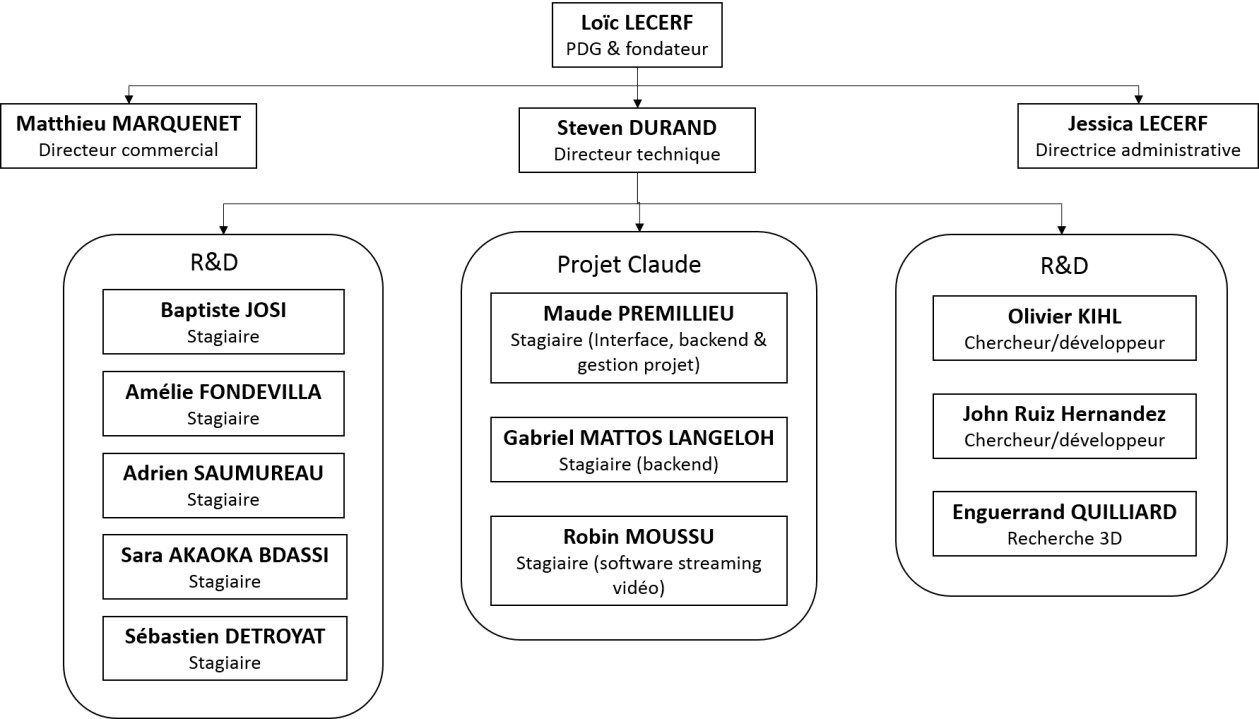
\includegraphics[width=\textwidth]{organigramme.jpg}
  \label{fig:organigramme}
  \caption{organization chart of \smu}.
\end{figure}

\chapterimage{Raspberry_Pi_2.jpg}
\chapter{Goal of the internship}
%% Présenter de manière concise et intelligible par une personne non spécialiste du
%% domaine la problématique de votre stage et bien définir l¿existant :
%% (environ 5 pages)
%% le problème à résoudre
%% les objectifs précis attendus 
%% l¿état de l¿art des solutions existantes et des contraintes fi xées par 
%% l¿entreprise
%% votre solution motivée à partir de l¿analyse ci-dessus

\section{The \claude{} project}

I have worked together whith Gabriel and Maud, two others interns. Our goal was
to grab videos from customers' cameras, and to analyse them on \smu's server
inside the cloud. At \smu, we were the \claude{} department (it's a pun with
\textit{cloud computing} with a big french accent $:$-$)$ ). During our
intership, we worked in the same office, so we were able to exchange a lot.

Even if Oliver Kilh was my tutor, in facts it was Steven Durand and Loïc Lecerf
who suppervise me and the others interns of the \claude{} project.

My initial goal was to create a software that can stream a video from all type of
devices to the servers of \smu, where it will be analysed. To be more specific,
I had to support all type of webcam, on \linux, \win{} and \mac, smartphones
(\android, \ios), and ip cameras.

Gabriel goal was to create the softwares used on the server. Thoses sofwares
have to receive the video stream, and analyse them using the library developped
by \smu.

Maud has created the web interface. That website is the place where customer can
access to the results of their analysis and where they can administrate their
cameras (the clients have to pay a subscription for all their camera, and the
type of analysis they have chosen).

\section{Technologics choises}

Our goal (Gabriel, Maud and me) was to select the appropriate technology for
what we have to do. To be more specific:
\begin{itemize}
\item How to capture the images
\item How to encode them
\item How to send them to \smu{} server.
\end{itemize}

And furthurmore
\begin{itemize}
\item How to etablish connection between clients' software and \smu{} servers
\end{itemize}

Our first task was to learn how video are streamed in general. That part is
explained in details later (in the section~\ref{sec:technologies}). The objective
was to found witch protocols are used for grapping encode and send image. Of
course it was not in our plan to reivent the well, so we also add to choose a
library that implement thoses protocols.

Our second goal was to define how our sofware will exchange informations. Since
clients machine, and \smu{} server are all links to internet, we have choose to
use http request. We have defined all messages we can send, and their
structure. The methodology and the result is explained in the
section~\ref{sec:communication}.

\section{Plateforms}

As I said, my personnal goal was to write a software that could be run virtualy
everywhere. To be more specific, my initial targets were \linux{} (on PC, and
embedded devices like \rpi or \bbb), \win, \android, \mac{} and \ios. It was a
bit too ambitious, so the last two were dropped.

All employees in \smu work on ubuntu (a \linux{} distribution), so I have first
developped my solution for linux, keeping in mind that I will have to port it
after, so I never use plateform specific stuff. Then I port it to linux arm (I
have test it on \rpi{} and \bbb). After that, I try to create an \android{}
application, and finnaly for \win.

I was requested to write my software in \cpp. As a consequence of using native
language, my build system has to be able to create executable for all
plateforms. I have choose to use \cmake{} as build system, since \cmake{} was
already use in the company.

\section{Synthesis}

Since I have to support a very heterogeneous set a plateform, I had to be very
generic.

The main complicated part was to make tradeoff between performance required for
video encoding and the available bandwith. To lower the required bandwith, we
can use a better compression algorithm, however better algorithm mean highter
compression time, so worst lattency, and higher cpu usage. On slow CPU hardware
(smartphones and embedded devices like \rpi{} and \bbb{}) it was a real
challenge to found the right algorithm.

The results of the analisys of our needs for the \claude{} project have lead to
the sofware organization presented on figure~\ref{fig:architecture}. That figure
is exclacted from the documentation Gabriel has wrote. To be more clear, what I
will later call \textit{http gateway} is the \textit{serveur HTTP}. The \textit{source} is anything
with a webcam (a pc, an embeded device, or a smartphone).

My contribution on the project was the source, and the specification of the
communications between HTTP gateway and streaming and analysis server. Gabriel
have worked on the video \& analisys server, and Maud on the rest (her intership
was longer).

\begin{figure}
  \centering
  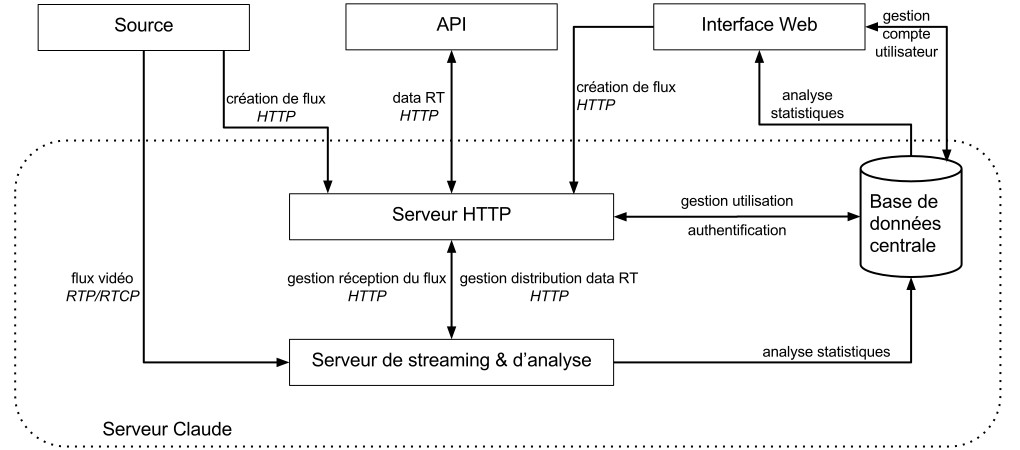
\includegraphics[width=\textwidth]{architecture.jpg}
  \label{fig:architecture}
  \caption{presentation of the \claude{} project structure}.
\end{figure}

\chapterimage{webcams.jpg}
\chapter{Methodology and implementation}
%% Décrire votre méthodologie de travail pour la mise en ¿uvre de votre solution 

\section{Organisation}

During all my intership, I had two small meeting per week (called \textit{point
claude}) with Steven Durand and Loïc Lecerf. The others interns of the \claude{}
project (Maude and Gabriel) were also there. During thoses meeting, we presented
the work we had done since the last time, and then we decide what to do next.
Since none of the employees of \smu{} have look our code during our intership (as
least for the \claude{} project, it was their only way to know what we were
doing.

Our general methodology was to quicly have something that work somewhere, and
then improve it by small iteration to make it work everywhere in all conditions.
As a consequence, we first test something on our machine, then using multiple
machine in local network, and finaly on the cloud.


\section{Technologies used}
\label{sec:technologies}

The main challenge of that internship was to found the right technology to
achieve the goal that I have been entrusted.

\subsection{Network protocol}

Firstly, we (Gabriel and me) have worked together to find the appropriate
protocol for video streaming. We have conclude that \rtp{} is a good choise.
That was motivate because \rtp{} can be easily replaced by \rtsp{} that work in
a similar way, but with encryption. Furthurmore, it can be use in tandem with
\rtcp, witch carry informations on the stream (like framerate, lag, and others
usefull informations to analyse the quality of the stream).

Select the right protocole is of course not enough, and since we have planed to
support multiples plateform, we have search implementations that match this
requirement. \ffmpeg{} (and his fork \avconv), \vlc{} and \gstreamer{} where good
quandidates. \vlc{} was quicly avoided, because it has too much code that we do
not need. It was nevertheless usefull for testing purpose. In July, we have used
\ffmpeg/\avconv, but we finally found that \gstreamer{} as better performance
results.

\subsection{Video encoding}

Having the right network protocol is still not enough. We had to choose an
encoding that fit our needs. What we want is something fast to encode,
because the client program can run on small hardware, and because low latency
was unavoidable. The resulted stream has also to be lightweight, because we
could not assume that \smu's client will have a fast internet connection.

All our tests have been first made on LAN, so \mjpeg{} was a very good
quandidate. It's just a sequence of \jpeg{} images, so it is realy, realy fast
to encode it, even on small hardware. As a direct consequence, the delay was
excellant. However when we have made the firsts real tests using a server
somewhere on the cloud, we have discover that the amount of data needed for the
transmission was too hight. So we had to choose something else less eager in
bandwith. We have tested \mpeg{} and \vpx, and we have choosen the later.

\subsection{Communication between devices}
\label{sec:communication}

At this point we knew how to grab images, encode them, and send them to a
server. It's cool, but we need something to ask the permission the server. We
choose to simply use http request. \curl{} was a good initial choise, since it
is a very powerfull library. However, in the optique of minimizing dependances,
I finally use \happyhttp. The request are formating is \json.

*** exemple ici

\section{Minimize the dependency}

One of my objective was to create a sofware whose source code is really
portable. For making that task easier, my tutor ask me to minimize the number of
dependencies, and their complexities.

\subsection{Prototyping}

When I was prototyping, I have used some python and shell scripts to work
faster. Since we cannot assume that thoses languages are installed on our client
machine, my tutor ask me to use native code (to be more specific \cpp). Binary
package are not transfereable across operating system and cpu, so I had to
generate binaries for all targets.

In July, I have wrote a software that did the work, but with too many
dependencies. I had used \boost{} for arguments and json parsing, and \curl{}
for http request. I have also used \gstreamer{} for video (grab image, compress
using \vpx{} and send using \rtp/\rtcp). Only the last was a requiered
dependency.

\subsection{Reducing complexicity}

Removing \boost{} and \curl{} was too complicated, so I re-write my software,
but much faster than the first time, since I already know what I want to do, and
how to do it.

To replace \boost{}, I have wrote a minimal \json{} parser (for the sub-part of
json used for the communication between the client and the http gateway).
To parse the arguments provided to the program, I have made a manual read of
the arguments on \verb+argv+. Of course my own code have less possibilities than
\boost{}, but it was less complex, and that was what I was asked for.

With the similar optique, I have replaced \libcurl{} by \happyhttp. That second
library is only one small source file, so it is easier to embed it. Furthurmore
the employees of \smu{} were already using it. With some take back, I think that
using \libcurl{} during the prototyping was a good idea. Indeed it had help me to
understand the errors easily when we (Gabriel and me) were creating the http
protocol between the client software and the http gateway.

Despite everything my main dependency was etheir \gstreamer{} or
\ffmpeg/\avconv. Since they are both as complex, it was not an arguments in
favor of one or another. At the end, \gstreamer{} (and it's own dependencies) is
the last remaining in my code, even if it is the most complicated.

\section{Solving problems}

During my intership, I have wasted some time because at some point I was stuck,
and I had not enough method to find the right solution in a short time. Making
pair-programming was a good idea, but we did not use it enough for my taste.

Sometime, when I was stuck, I left my desk, to help someone else, and when I
came back that person help me back. In general, that save us both a lot of time,
because, it help us to take a more global view on what we were doing. The key
point of that is that explaining to someone else our problem help us to
formalize it.

\chapterimage{technology-computer-chips-gigabyte.jpg}
\chapter{Results}

\section{Technologies used}

\subsection{Build system}

I have developped a build system based on \cmake. It was choosen because it is
cross plateform (that was obviously required), and powerfull enough to fit my
need. I also wrote a small python script to call \cmake{} more easyly. I have
developped it when I was trying to make cross compilation. So in one command, I
build the whole program for all architecture. At the end, I used it just as an
helper.

XXX
cross-compillation
Our initial goal was to have a cross-plateform build system. In that ideal
scenario, when I want to create a new release of my software, I have

The build process for \linux, on intel and arm device or for \win{} is quite
similar (except some fiew \#ifdef), so the build system is the same (we use
\cmake). On \android{} however, The main has to be written in java. So, I have
used \jni{} to build my \cpp{} codebase and linked it to java. So I can share my
work also on that plateform.

\subsection{Grab image and send video}

\gstreamer{} pipeline
\ffmpeg/\avconv{} work similary.

\subsection{Android}

Android sofware has to be in java. Since my work was done in \cpp, I have use
\jni, that allow me to call \cpp code from java. I have also use tha \android{}
sdk and ndk as well as the gstreamer sdk. Using thoses software tools as allow
me to easily start to port my software. However, some differences in the usage
of \gstreamer{} on \android{} have made the developpement more difficult, and I
had not enough time to finish it.

\subsection{Installer}

In the optique of being as simple as possible for the user to test that sofware,
I had to design my sofware in a way it could be used without installation.
(\fpm{} was initialy used to create real .deb package)

\section{Conclusion}

To sum up, at the end of my intership, I have wrote a sofware that can compile
and run on multiple plateforms~: \linux{} (both intel and arm) and \win. A lots
of work have also be done for \android, but not everything have been finished.
My program is able to ask the htpp gateway the autorization to start the stream.
Then it grab images, compress them using \vpx{} encoding, and send them using a
\rtp{}/\rtcp{} stream. All that is done using a gstreamer backend. The program I
wrote still need more tuning to be faster, especially on embedded hardware.

%\chapterimage{Pink_flowers.jpg} % Table of contents heading image
\chapterimage{binary.jpg}
\chapter{Personnal conclusion}

To sum up, the keys points of my intership were:
\begin{multicols}{2}
\begin{itemize}
\item design a sofware architecture
\item define witch protocols will be used and how
\item create a robust build system
\item understand the link process
\item how to build for multiple target (\linux{} arm and intel, \win, \android)
\item try to have cross compilation
\end{itemize}
\end{multicols}

The part that motivate me the most was designing the communication protocol.
When designing a protocol, we have to take care of making it both expressive and
easy to parse/understand. I found that the result is pretty clean, and it was a
good experience to work with Gabriel and Maud under the direction of Steven
Durand and Loïc Lecerf.

The major amount of work was the build process and its fine details. Building
for one architecture is realy easy, however when we want to support many more
system, it become more complicated. \cmake{} was realy usefull to simplify that
task. What was too complicated for me was cross-compiling with many dependencies
at the same time, using static link. Despite everything, I have learned a lot of
that process.

To summurize, that intership was really instructive, and I feel that I have a
finer understanding of the \cpp{} build process.

\end{document}
\end{document}
